% Kapitel "A Delta-Learning Head for Level-of-Theory Correction".
% Kopie aus der Thesis, hier abgelegt am 2026-09-07, damit der Text im Repo
% verfuegbar ist. Nicht vom Repo geprueft; Zahlen stammen aus der
% Delta-Pipeline, nicht aus results/*.csv.
%
% Bekannte Stellen im Entwurf:
%   - "Protocol B: the surface" und "The earlier head" (mit Tabelle
%     tab:delta-neb-results, Figuren fig:neb-results, fig:rmsd-parity und
%     Tabelle tab:delta-audit) stehen ZWEIMAL hintereinander.
%   - 2026-09-12: \section{Motivation} (Absaetze 1-4) nach docs/introduction.tex
%     verschoben; Gleichungen und Architektur eroeffnen jetzt \section{Method}.
%
% ============================================================
%  Chapter: A delta-learning head for level-of-theory correction
%  Requires: booktabs not used; \hline style consistent with theory chapter
%  Bib keys used that may need adding: batatia2022
% ============================================================
\usetikzlibrary{positioning, arrows.meta}

\chapter{A Delta-Learning Head for Level-of-Theory Correction}
\label{ch:delta}

\section{Construction and Training}
\label{sec:delta-overview}

This chapter answers RQ1, whether a model can be lifted to a higher
level of theory by relabelling only a subset of its training data.
About 80\,000 geometries, under 1\,\% of the dataset, are relabelled;
the paths
themselves stay where Transition1x relaxed them, at
\mbox{$\omega$B97X/6-31G(d)}, and are not re-optimised at the new
level. A MACE model is trained on Transition1x
(Section~\ref{sec:mace-training}), and a small correction head on top
of it (Section~\ref{sec:delta-architecture}) learns the difference
between the two levels,
%
\begin{equation}
\Delta(\mathbf{R}) \approx E_{\omega\text{B97M-V/def2-TZVP}}(\mathbf{R}) - E_{\omega\text{B97X/6-31G(d)}}(\mathbf{R}) .
\label{eq:delta-def}
\end{equation}
%
This is feasible with so little data because $\Delta$ is nearly
constant within a reaction ($\approx 3$\,eV per molecule in magnitude,
$\approx 0.09$\,eV within-reaction standard deviation,
Section~\ref{sec:delta-data}): a smooth offset is far easier to learn
than the potential energy surface itself.

The target level is \mbox{$\omega$B97M-V/def2-TZVP}, not coupled
cluster, for one reason: the head is trained on energies and forces at
80\,000 geometries, and CCSD(T) gradients cost of order $N^7$
(Section~\ref{sec:background-beyond}). The largest reactive dataset at
that level holds 3119 configurations~\cite{allen2026}.

Two names are used throughout this thesis. MACE is the base model: a
MACE model trained on Transition1x at \mbox{$\omega$B97X/6-31G(d)}.
MACE+$\Delta$ is the same model with the correction head attached; it
approximates \mbox{$\omega$B97M-V/def2-TZVP}. Base model and
correction head combine into one corrected potential; the superscript
denotes the level of theory a prediction approximates:
%
\begin{equation}
E_{\text{MACE}+\Delta}^{\,\omega\text{B97M-V/def2-TZVP}}(\mathbf{R})
=
E_{\text{MACE}}^{\,\omega\text{B97X/6-31G(d)}}(\mathbf{R})
+ \Delta^{\,\omega\text{B97M-V/def2-TZVP}\,-\,\omega\text{B97X/6-31G(d)}}(\mathbf{R})
\label{eq:delta-energy}
\end{equation}
%
\begin{equation}
\mathbf{F}_{\text{MACE}+\Delta}^{\,\omega\text{B97M-V/def2-TZVP}}(\mathbf{R})
=
\mathbf{F}_{\text{MACE}}^{\,\omega\text{B97X/6-31G(d)}}(\mathbf{R})
- \nabla_{\mathbf{R}}\Delta^{\,\omega\text{B97M-V/def2-TZVP}\,-\,\omega\text{B97X/6-31G(d)}}(\mathbf{R})
\label{eq:delta-forces}
\end{equation}
%
The correction forces are analytic gradients of the head's output.

Architecturally, this sum is a single network
(Figure~\ref{fig:mace-delta-arch}): the frozen MACE encoder with two
readout heads --- the original energy readout, yielding
$E_{\text{MACE}}$, and the newly trained correction head, yielding
$\Delta$ (Section~\ref{sec:delta-architecture}). The forces in
Eq.~\eqref{eq:delta-forces} are computed as the exact derivative of the
corrected energy, so energies and forces are consistent with each
other, and MACE+$\Delta$ can be used wherever MACE can: for
single-point predictions or as the potential driving a NEB
optimisation.

MACE+$\Delta$ is built in two steps. First, a MACE base model is trained on
Transition1x (Section~\ref{sec:mace-training}) --- the model whose level of theory we upgrade. It
must exist first, because it provides both things the correction builds on:
the baseline prediction $E_{\text{MACE}}$, and the frozen per-atom
representation of molecular geometry from which the correction head reads.
The head is a new, additional readout with its own 131{,}136
parameters\footnote{More than MACE's own energy readout (17{,}442): the head
is wider (64 vs.\ 16 channels) and reads the scalar features of both encoder
layers rather than one. It needs the extra capacity because it reads frozen
features that were never shaped for its task, whereas MACE's readout was
trained jointly with the encoder.}; it does not replace or retrain any part
of MACE. All original weights, encoder and energy readout alike, stay frozen,
so $E_{\text{MACE}}$ is identical before and after.

MACE~\cite{batatia2022} was chosen for both roles at once: it is among the most
accurate and data-efficient MLIP architectures, and its encoder produces a
rich per-atom representation of the chemical environment that a second
readout can reuse without retraining. Figure~\ref{fig:mace-delta-arch} shows
the resulting structure: one shared encoder, two readouts, one forward pass.

\begin{figure}[t]
  \centering
  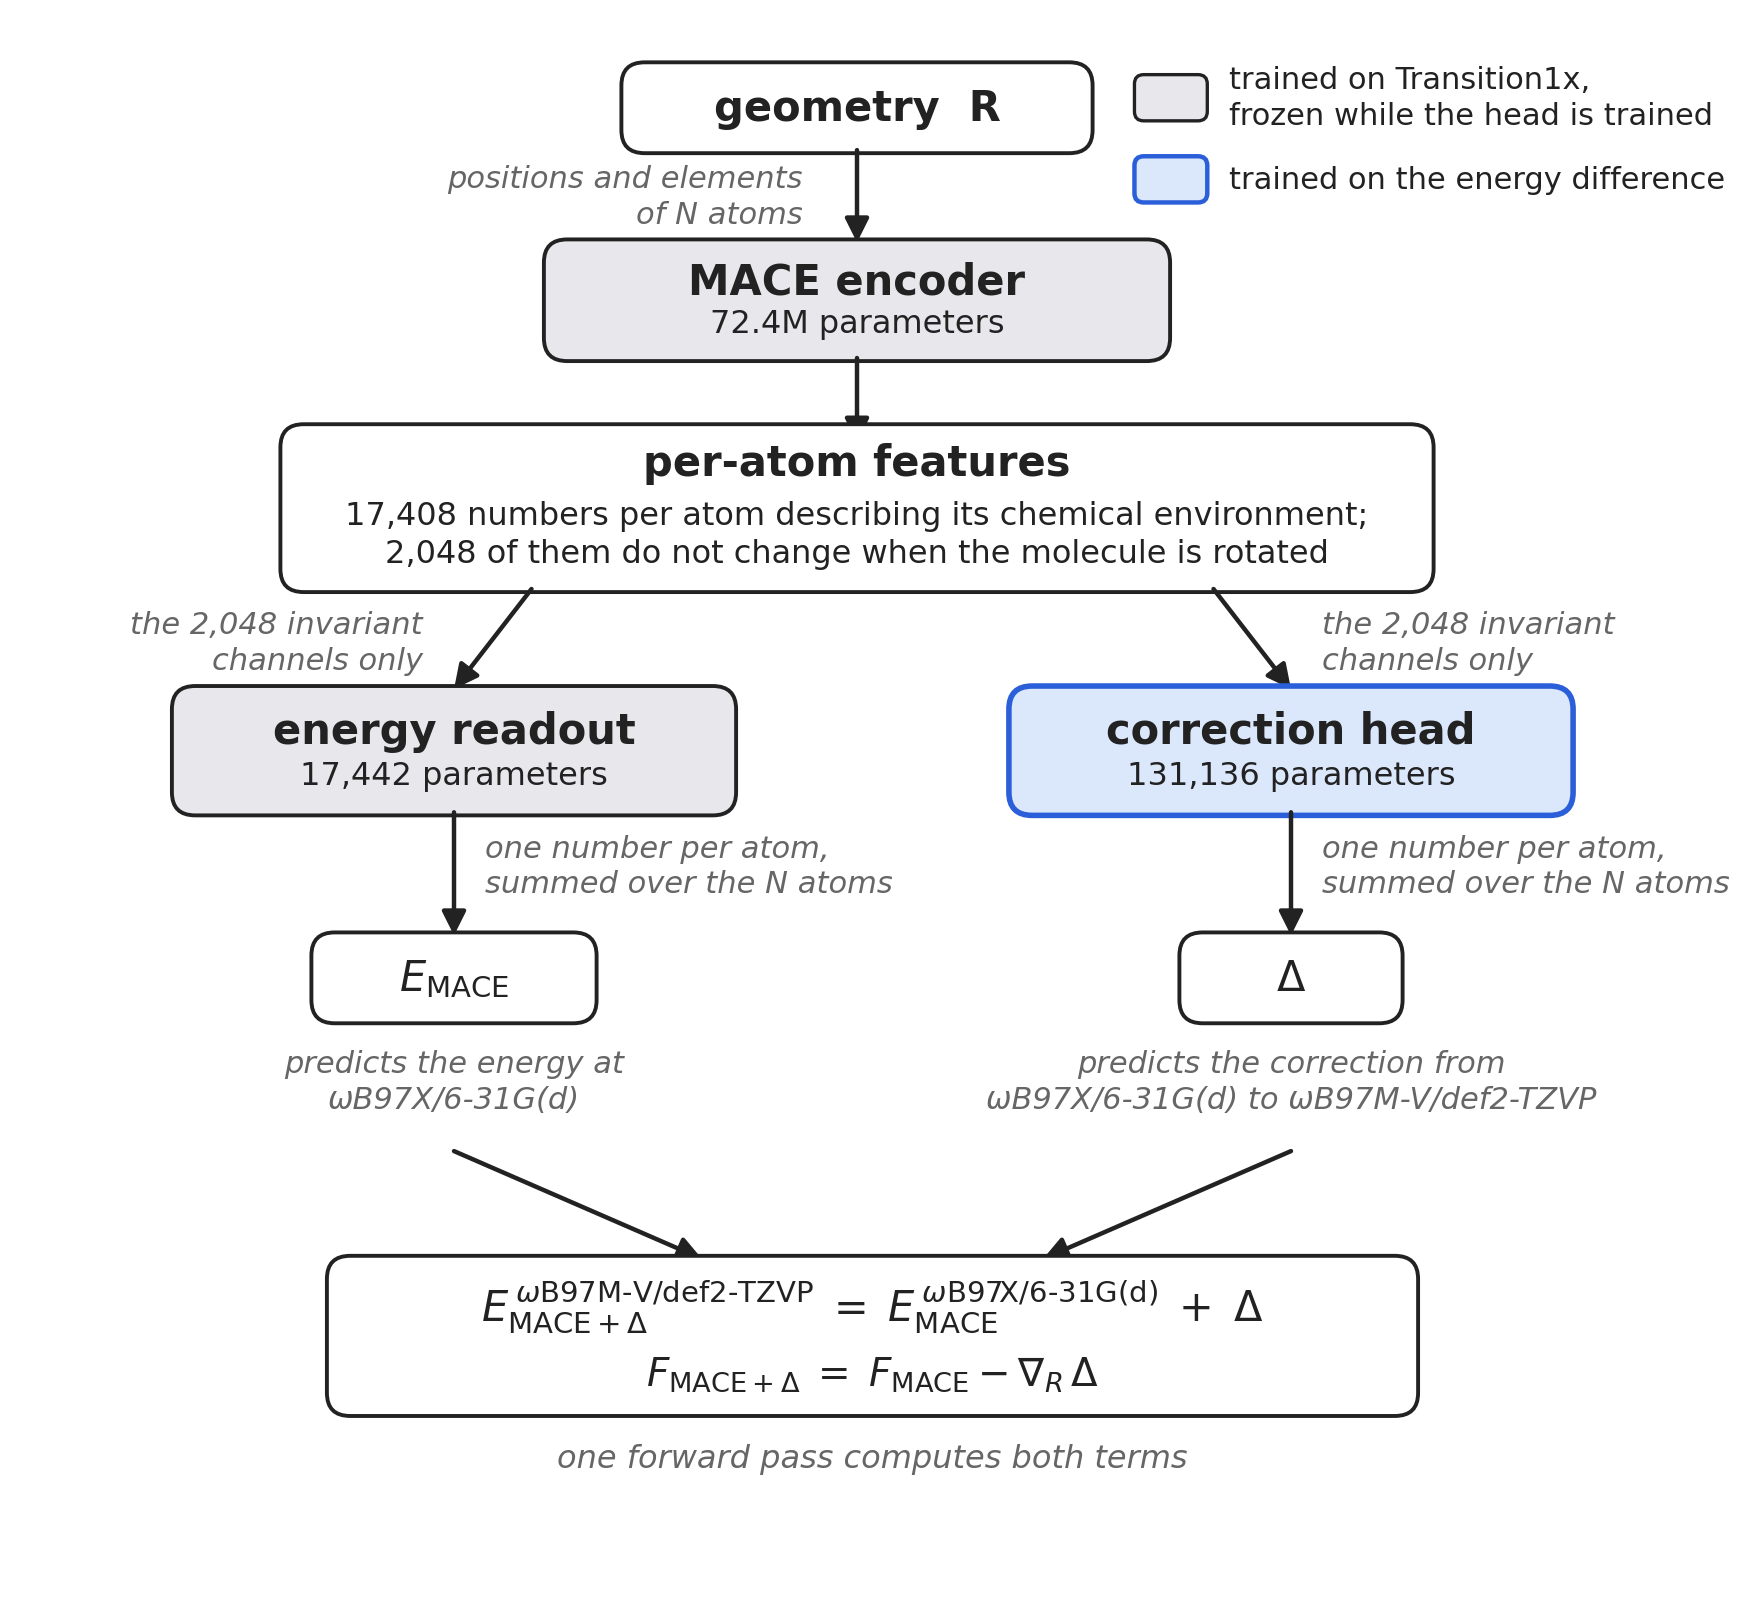
\includegraphics[width=0.95\textwidth]{Pictures/mace_delta_architecture_v4.png}
  \caption{Structure of MACE+$\Delta$. One forward pass through the frozen
  encoder produces the per-atom features; 2{,}048 of the 17{,}408 numbers per
  atom are rotation-invariant. Both readouts read these invariant
  channels: the original energy readout predicts the energy at the
  baseline level, the correction head the shift to the target level.
  Both output one number per atom, summed over atoms, and the sum of the two
  results is the corrected prediction.}
  \label{fig:mace-delta-arch}
\end{figure}


\subsection{Base model: MACE trained on Transition1x}
\label{sec:mace-training}

We trained a MACE model from scratch on the Transition1x training split, using
the dataset's \mbox{$\omega$B97X/6-31G(d)} energies and forces as targets. A full
pass over the ${\sim}9$ million training geometries per epoch is impractical,
so each epoch used a random subsample of 100{,}000 geometries. Training ran for
362 epochs, i.e.\ 36.2 million samples --- about four passes over the full
dataset. Table~\ref{tab:mace-settings} lists the settings.

\begin{table}[htbp]
  \centering
  \caption{MACE architecture and training settings.}
  \label{tab:mace-settings}
  \begin{tabular}{ll}
    \toprule
    Setting & Value \\
    \midrule
    Architecture & MACE (ScaleShiftMACE), 2 interaction layers \\
    Channels / max.\ $L$ / correlation order & 1024 / 3 / 3 \\
    Cutoff radius & 6.0\,\AA{} (Bessel, 16 radial basis functions) \\
    Total parameters & 72{,}390{,}332 \\
    Loss & Huber ($\delta = 0.01$), energy\,:\,force weight 1\,:\,100 \\
    Optimizer & AdamW, learning rate $10^{-3}$, gradient clipping 10 \\
    Scheduler & ReduceLROnPlateau, factor 0.8, patience 10 \\
    Batch size & 64 \\
    Geometries per epoch & 100{,}000 (random subsample) \\
    \bottomrule
  \end{tabular}
\end{table}

On the Transition1x test split the model reaches a force RMSE of
81\,meV/\AA, compared to 136\,meV/\AA{} for the PaiNN model that the
Transition1x authors trained on the same data~\cite{schreiner2022}.

\subsection{Correction head: architecture}
\label{sec:delta-architecture}

The head works on the features of the frozen encoder. For every atom, the
encoder produces 17{,}408 numbers; 2{,}048 of them are rotation-invariant
scalars (1{,}024 from each of the two layers, Table~\ref{tab:mace-features}),
the rest rotate with the molecule. The head reads only the scalars: $\Delta$ must not change when the
molecule is rotated, and an output that does not rotate can only be
built from inputs that do not rotate. The directional features still
matter, but only inside
the encoder, where the tensor products of one layer turn them into the
scalars of the next. A small MLP (64 channels, SiLU, 131{,}136 parameters)
maps the scalars to one contribution per atom; the sum over atoms is
$\Delta(\mathbf{R})$. Forces follow by differentiating $\Delta$ through head
and encoder, so the corrected potential is conservative.



\paragraph{An earlier version of the head.} \emph{It declared its input
incorrectly: it labelled 1{,}024 direction-dependent components as scalars, put all of its weights on
them, and ignored the true scalars. As a result, $\Delta$ changed when the
molecule was rotated, by 212\,meV on average across the benchmark transition
states. We found the error by counting parameters: the head had
$65{,}600 = 1024 \cdot 64 + 64$ of them, which means it read only 1{,}024 of
its input dimensions; the stored weights and the MACE source code confirmed
it. We corrected the declaration and retrained the head on unchanged data.
All results in this chapter use the corrected head;
Section~\ref{sec:delta-results} compares both versions.}


\subsection{Training data}
\label{sec:delta-data}

The head is trained on geometries for which both level of theory labels are known.
Transition1x already stores the $\omega$B97X/6-31G(d) energies and forces;
we recompute the same geometries, unchanged from Transition1x, at
$\omega$B97M-V/def2-TZVP and subtract:
\begin{equation}
  \Delta E = E_{\omega\text{B97M-V/def2-TZVP}} - E_{\omega\text{B97X/6-31G(d)}},
  \qquad
  \Delta \mathbf{F} = \mathbf{F}_{\omega\text{B97M-V/def2-TZVP}} - \mathbf{F}_{\omega\text{B97X/6-31G(d)}}.
\end{equation}
These differences are the training targets.

We sampled 5{,}000 reactions at random from the Transition1x training split
(fixed seed) and selected 20 of the ${\sim}950$ path geometries per reaction.
The selection follows the shape of the reaction path. A path runs from the
reactant up to the transition state and back down to the product; the
transition state is the geometry with the highest $\omega$B97X energy. We
cut the path into four stretches --- the flat region before the climb, the
climb up to the transition state, the descent just after it, and the
remainder down to the product --- and picked five evenly spaced geometries
from each (Figure~\ref{fig:stratified-sampling}). The two stretches at the
barrier are short, so half of all selected geometries lie close to the
transition state, and the transition state itself is always among them. A
uniform selection of 20 geometries would give no such guarantee.

We recomputed each selected geometry with a single-point
energy-and-gradient calculation at $\omega$B97M-V/def2-TZVP,
restricted\footnote{Restricted was the program default for a singlet
input, not a deliberate choice; what the choice implies is the subject
of Chapter~\ref{ch:mr}, and why the default persists is discussed in
Chapter~\ref{ch:conclusion}.} (ORCA, RIJCOSX, TightSCF). For three reactions some of these calculations did not complete; we
discarded reactions with fewer than 15 finished geometries, leaving 4{,}997
reactions and 80{,}592 training geometries, each with an energy and a force
target. This amounts to ${\sim}100{,}000$ DFT calculations, 3--4 days on the
cluster, and under 1\,\% of the dataset (Chapter~\ref{ch:introduction}).
These 80{,}592 geometries with their energies and forces are the
training set of the correction head.

For validation we relabelled 225 reactions from the Transition1x validation
split in the same way (10{,}600 geometries, 2{,}240 of them with force
labels); Section~\ref{sec:delta-training} describes how they are used.

\begin{figure}[htbp]
  \centering
  
\includegraphics[width=0.9\textwidth]{Pictures/stratified_sampling.png}
  \caption{Stratified sampling of training geometries along a reaction path.
  The path is cut into four stretches at one quarter of the path, at the
  transition state (highest-energy frame), and at the midpoint of the descent.
  Five evenly spaced geometries are taken from each stretch. The stretches
  adjacent to the transition state are short, so the selected geometries
  cluster around the barrier; the transition state itself always lies on a
  stretch boundary and is included.}
  \label{fig:stratified-sampling}
\end{figure}

\subsection{Training the correction head}
\label{sec:delta-training}

The head is trained with the loss
\begin{equation}
  \mathcal{L} = \mathrm{Huber}(\Delta E) \;+\; \lambda_F\,\mathrm{Huber}(\Delta \mathbf{F}),
\end{equation}
with all settings listed in Table~\ref{tab:delta-training}. The force weight
$\lambda_F$ was selected by a sweep over $\{0.5, 1.0, 2.0\}$; $\lambda_F = 2.0$
gave the lowest validation force loss and is used for the final head. The
sweep was run on the earlier version of the head; after the audit of
Section~\ref{sec:delta-architecture}, we retrained the corrected head from
scratch with these exact settings and $\lambda_F = 2.0$ on unchanged data.
Training takes about six hours on a single GPU, negligible next to the DFT
relabelling of Section~\ref{sec:delta-data}.

\begin{table}[htbp]
  \centering
  \caption{Training settings of the correction head.}
  \label{tab:delta-training}
  \begin{tabular}{ll}
    \toprule
    Setting & Value \\
    \midrule
    Loss & Huber, $\delta = 0.1$\,eV \\
    Force weight $\lambda_F$ & 2.0 (sweep over 0.5 / 1.0 / 2.0) \\
    Optimizer & Adam, learning rate $10^{-3}$ \\
    Batch size & 64 \\
    Geometries per epoch & 10{,}000 (random subsample) \\
    Epochs & up to 200; stop when learning rate falls below $10^{-6}$ \\
    Scheduler & ReduceLROnPlateau, factor 0.5, patience 10 \\
    Scheduler signal & loss on a fixed sample of 1{,}024 validation geometries \\
    Checkpoint criterion & force loss on the 2{,}240 force-labelled validation geometries \\
    \bottomrule
  \end{tabular}
\end{table}

The last two rows use different validation quantities on purpose. The
scheduler lowers the learning rate when the total loss on a fixed
sample of 1{,}024 validation geometries stops improving. The
checkpoint that is kept is the epoch with the lowest force loss on
the 2{,}240 force-labelled validation geometries, because the head is
deployed to drive NEB optimisations, and there the forces are what
matters.


\subsection{Evaluation protocol}
\label{sec:delta-protocol}

The model is built; now we test it. We run $\omega$B97M-V/def2-TZVP reference
calculations on reactions from the Transition1x test split, select 30 of
them stratified by multireference character, and compare MACE and
MACE+$\Delta$ against the reference in two ways: as single points on fixed
reference geometries, and with the model driving the NEB optimisation
itself.

\paragraph{Reference.}
We run a restricted $\omega$B97M-V/def2-TZVP CI-NEB for each reaction of the Transition1x
test split. This level of theory is the natural reference: it is exactly
what MACE+$\Delta$ is trained to approximate. Each converged run yields the
quantities we later compare against: ten geometries along the reaction path,
each with its $\omega$B97M-V/def2-TZVP energy and forces; the transition-state geometry (the
highest image of the band); and the reference barrier that follows from the
energies. A model can therefore be tested on every level --- energies and
forces at given geometries, the barrier height, and the transition-state
structure it finds itself. For 279 of the 287 test-split reactions the NEB
converges; the remaining eight are discarded from every step that follows.
One limitation applies. The reference is restricted DFT, a
single-determinant description, and for reactions with strong
multireference character that description is itself inaccurate.
Agreement with it then shows that the head has learned what it was
trained on, the restricted $\omega$B97M-V/def2-TZVP surface, not that
the prediction is closer to the true surface.

\begin{table}[htbp]
  \centering
  \caption{Settings of the $\omega$B97M-V/def2-TZVP reference CI-NEB.}
  \label{tab:reference-neb}
  \begin{tabular}{ll}
    \toprule
    Setting & Value \\
    \midrule
    Level of theory & $\omega$B97M-V/def2-TZVP (def2/J, RIJCOSX, TightSCF; ORCA) \\
    Band & 10 images: reactant, 8 interior images, product \\
    Starting band & final $\omega$B97X/6-31G(d) NEB images from Transition1x \\
    Endpoint relaxation & BFGS, $f_{\max} = 0.05$\,eV/\AA \\
    NEB stage & ASE NEBOptimizer, $f_{\max} = 0.15$\,eV/\AA \\
    CI-NEB stage & climbing image on, $f_{\max} = 0.05$\,eV/\AA \\
    Step limit & 500 per stage \\
    Transition state & highest-energy image of the converged band \\
    \bottomrule
  \end{tabular}
\end{table}



\paragraph{Reactions stratified by multireference character.}
The correction head is expected to behave differently at high and low
multireference character, so the test reactions are grouped by it.
We therefore compute $N_{\mathrm{FOD}}$ at the
reference transition states (PBE/def2-SVP, Fermi smearing,
$T_{\mathrm{el}} = 5000$\,K; see Section~\ref{sec:background-beyond} for details), where we expect
the multireference character to be highest, rank the 279 reactions by it,
and select 10 high-MR reactions from the top of the ranking, 10 mid-MR
reactions spread across the middle, and 10 low-MR reactions from the
bottom. The 30 reactions are unimolecular CHNO reactions of 10 to 14 atoms,
all neutral singlets. None of them appear in the training or validation
data of the head or of the base model.

\paragraph{Evaluating performance on single-point predictions on fixed geometries.}
First, we want to test how accurate the single-point predictions are: energies, forces and
barriers. Whether a model also finds good geometries on its own is a
separate question and left to the NEB-driven evaluation. In this
fixed-geometry evaluation every method therefore computes single
points on the same fixed geometries, and no atom is moved.

We want to answer two questions. First: MACE is trained to approximate
$\omega$B97X/6-31G(d) --- does it reproduce $\omega$B97X/6-31G(d) energies and forces well?
Second: MACE+$\Delta$ is trained to approximate $\omega$B97M-V/def2-TZVP --- does
it reproduce $\omega$B97M-V/def2-TZVP energies and forces well? Both terms of
Eq.~\eqref{eq:delta-energy} are error sources, so both have to be
accurate on their own. The first question tests the base model; the
second tests the corrected model.

Both questions are evaluated on the same geometries: the ten images
of the converged $\omega$B97M-V/def2-TZVP reference band of each
reaction, 300 geometries in total, from reactant over the transition
state to product. Each geometry needs a reference value at both
levels. The $\omega$B97M-V/def2-TZVP energies and forces are those
of the NEB run itself. To also have $\omega$B97X/6-31G(d) energies
and forces, we compute them as single points on the same 300
geometries with ORCA.

Absolute energies at the two levels differ by a constant offset of
about 3\,eV per molecule. Per reaction, we therefore subtract each
method's energy at the reactant from its ten energies, which leaves
the energy profile along the path. We compare profiles image by image,
take the highest point of the profile as the barrier, and compare
forces image by image.

To summarise: this gives, for each of the 300 geometries, a reference
energy and force at both levels. From these we answer the two
questions about the single-point performance of the models: MACE
against \mbox{$\omega$B97X/6-31G(d)}, MACE+$\Delta$ against
\mbox{$\omega$B97M-V/def2-TZVP}, in energies, forces and barriers.

\paragraph{Evaluating performance on NEB driven TS search and barrier prediction.}
We want to test whether the models can do what they are built for: find a transition
state and a barrier on their own. The fixed-geometry evaluation cannot answer this. A model can predict accurate energies at
given geometries and still have a surface that is too rough to optimise on.

Each model runs the full workflow itself: it relaxes reactant and product,
then drives a CI-NEB with the same settings as the reference
(Table~\ref{tab:reference-neb}). We compare two outcomes. The barrier the
model finds is compared against the reference barrier. The transition-state geometry
the model finds is compared against the reference transition state, as
root-mean-square deviation (RMSD) over all atoms after Kabsch alignment. The first measures the energetics of the
surface, the second its shape.

\section{Results \& Discussion}
\label{sec:delta-results}

\paragraph{Evaluating performance on single-point predictions on fixed geometries: how well does MACE reproduce its target level $\omega$B97X/6-31G(d)?}
The first question was whether MACE reproduces its own target level
and therefore serves as a base that predicts the cheap level
accurately before the head corrects it. It does: on the 300 benchmark
geometries, MACE deviates from the $\omega$B97X/6-31G(d)
single points by 42\,meV in energy and 34\,meV/\AA{} in forces (force
cosine 0.95). For comparison, the two DFT levels differ by 112\,meV and
141\,meV/\AA{} ($\omega$B97X rows of Table~\ref{tab:delta-sp-results}). The
baseline error is three to four times smaller than the gap the head is
trained to correct.

This error still matters. Subtracting the target from Eq.~\eqref{eq:delta-energy} and
inserting $E^{\omega\text{B97X}}$ splits the error of the corrected model into
two parts:
\begin{equation}
\underbrace{E_{\text{MACE}+\Delta} - E^{\omega\text{B97M}}}_{\text{total error}}
=
\underbrace{\left(E_{\text{MACE}} - E^{\omega\text{B97X}}\right)}_{\text{baseline error}}
+
\underbrace{\left(\Delta - \left(E^{\omega\text{B97M}} - E^{\omega\text{B97X}}\right)\right)}_{\text{head error}} .
\label{eq:error-split}
\end{equation}
The head can only reduce the second term; the first passes through
unchanged. This bounds what the correction can achieve: MACE alone
misses its own level by 42\,meV on these geometries, that error
enters MACE+$\Delta$ unchanged, and the corrected model ends at a
total error of 56\,meV (next paragraph). Any further improvement
therefore has to come from the base model as much as from the head.


\paragraph{Evaluating performance on single-point predictions on fixed geometries: how well does MACE+$\Delta$ reproduce its target level $\omega$B97M-V/def2-TZVP?}
The second question was whether the correction brings MACE closer to the
target level. It does at low multireference character, and it
overshoots at mid and high. Table~\ref{tab:delta-sp-results} and
Figures~\ref{fig:barrier-errors} and \ref{fig:force-errors} show this by MR
tier.

All numbers that follow are deviations of MACE and MACE+$\Delta$ from
the $\omega$B97M-V/def2-TZVP reference on the 300 fixed geometries:
energies and forces image by image, and the barrier as the maximum of
the energy profile.

The forces are the clear win: they improve on all 30 reactions, in every
tier (force MAE against the reference, MACE $\rightarrow$ MACE+$\Delta$,
low, mid and high MR: 104 $\rightarrow$ 32, 152 $\rightarrow$ 53,
160 $\rightarrow$ 59\,meV/\AA). Figure~\ref{fig:force-errors} shows why. MACE's force error
against the reference is essentially the level gap itself, and the
correction removes most of it. The energies improve in every tier as well,
most strongly at low MR (86 $\rightarrow$ 30\,meV), only marginally at high
MR (89 $\rightarrow$ 83\,meV).

The barriers behave differently from tier to tier. On the low-MR
reactions the correction cuts the error
from 170 to 47\,meV and removes the bias of the level of theory gap ($+170
\rightarrow +21$\,meV): in Figure~\ref{fig:barrier-errors}, the orange
points move onto the reference line. On the mid- and high-MR reactions they
move past it, and the overestimation turns into an underestimation of
similar size ($-134$ and $-185$\,meV bias).

Eq.~\eqref{eq:error-split} splits the barrier bias of each tier into
two parts: the error of MACE against its own level, and the error of
the head against the true gap between the two levels.
Figure~\ref{fig:bias-decomposition} shows both. At low MR both are
small, and the corrected barrier lands on the reference. At mid MR
the base model misses its own level by $-91$\,meV and the head
overshoots the gap by $-43$\,meV; both push the corrected barrier
past the reference. At high MR the base model misses its own level
by $-192$\,meV, while the head reproduces the gap to within
$+7$\,meV: the overshoot there is the base model's error passed
through.\footnote{The average
over all 30 reactions (168 vs.\ 127\,meV,
Table~\ref{tab:delta-sp-results}) is misleading: it mixes a threefold
improvement on one third of the benchmark with a comparable deterioration
on another. The tiers carry the information. The off-scale reaction in the
mid panel, rxn0896, is a baseline failure, not a correction failure:
$\omega$B97X/6-31G(d) itself lies within 4\,meV of the reference, while MACE misses its
own level by 517\,meV.\label{fn:all30}}

\begin{figure}[htbp]
  \centering
  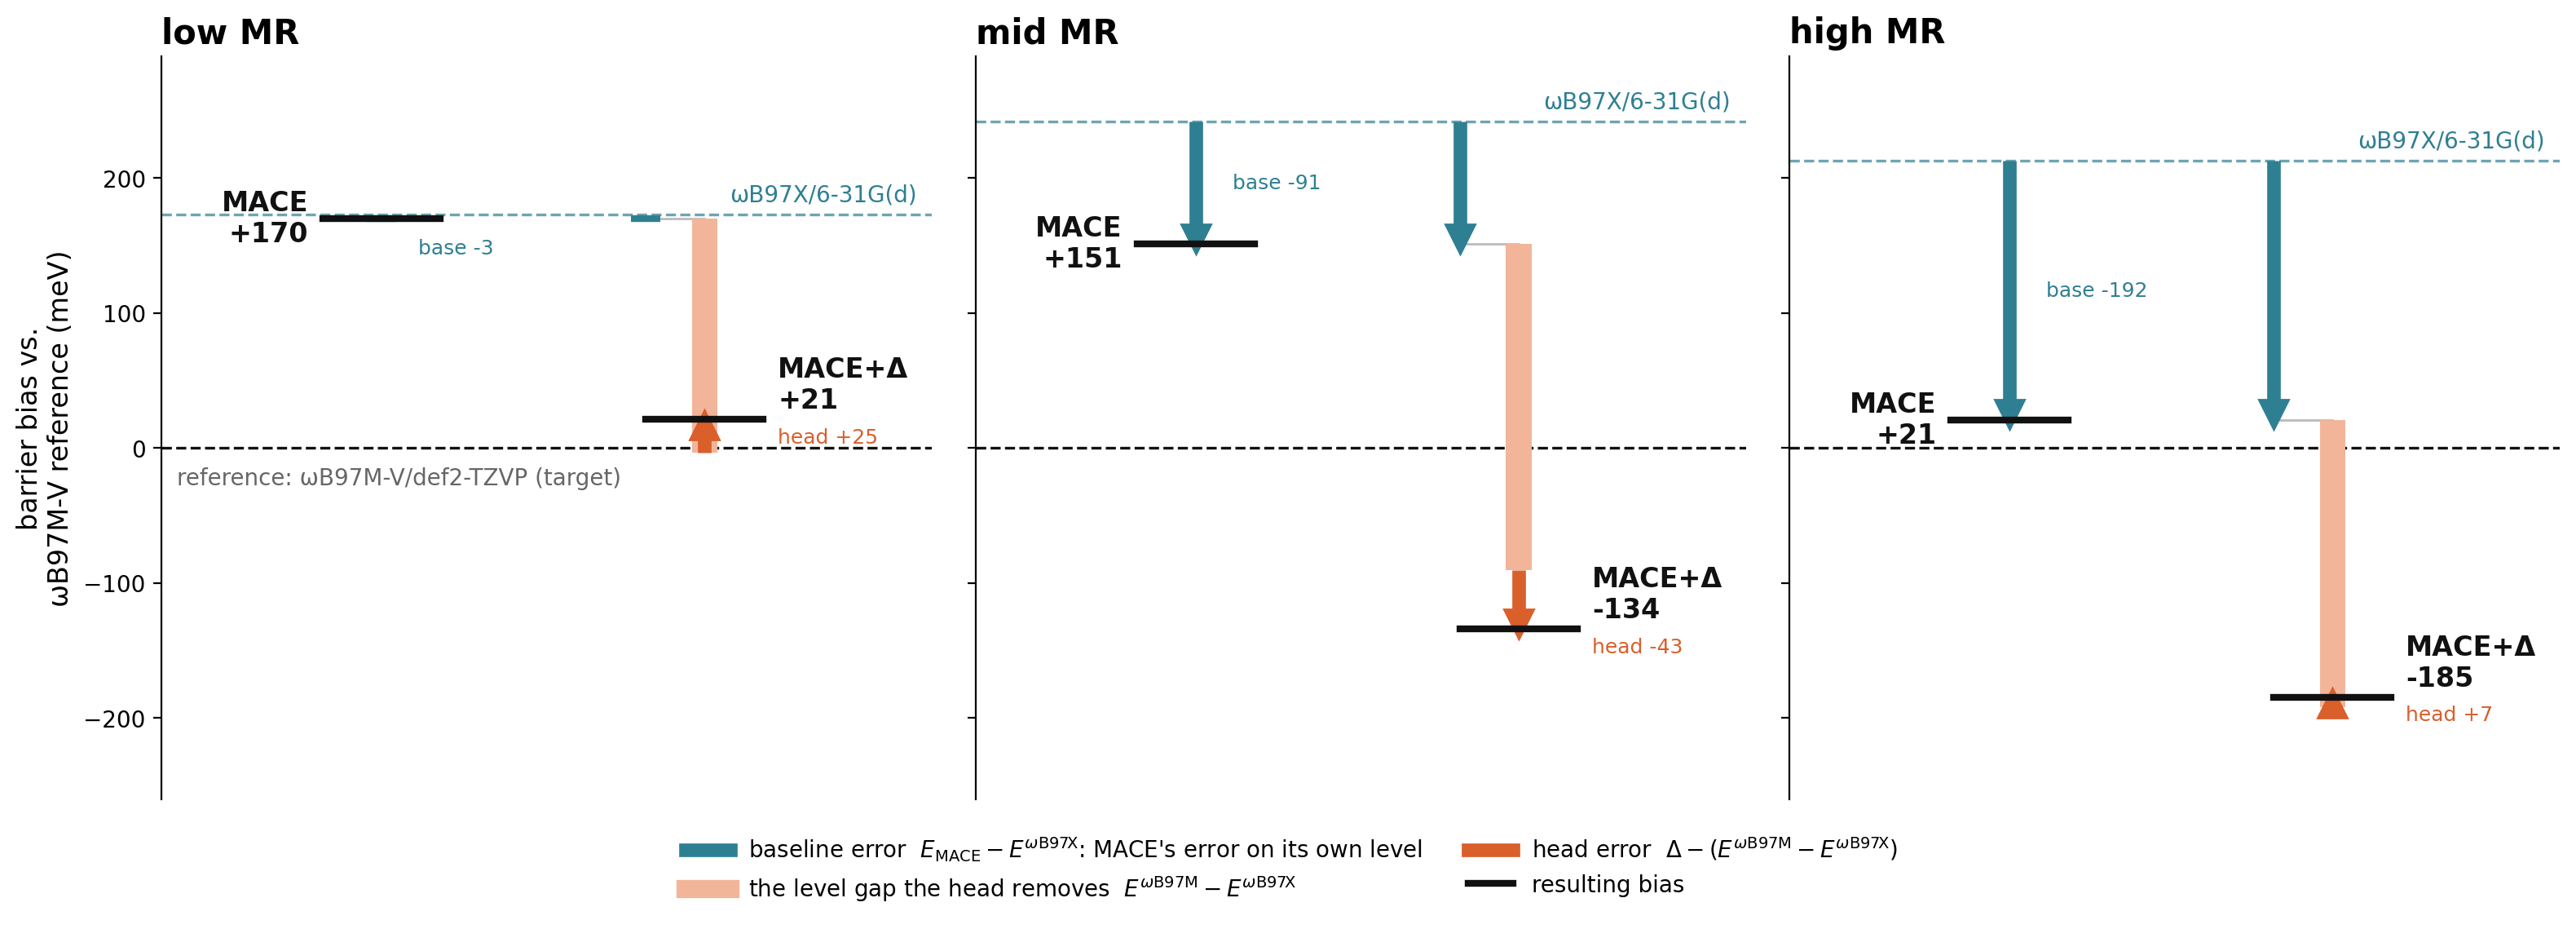
\includegraphics[width=\textwidth]{Pictures/bias_decomposition_v5.png}
  \caption{Barrier bias at fixed geometries, decomposed by
  Eq.~\eqref{eq:error-split}, per MR tier. Dashed lines: the
  $\omega$B97X/6-31G(d) level and the reference. Teal arrow: the
  baseline error of MACE against its own level; light orange: the level
  gap the head removes; dark orange: the head's error against that gap;
  black tick: the resulting bias, MACE on the left, MACE+$\Delta$ on
  the right. The head error stays small in every tier, the baseline
  error grows with multireference character, and at high MR bare MACE
  lands near the reference only because its baseline error cancels the
  level gap.}
  \label{fig:bias-decomposition}
\end{figure}


\begin{table}[htbp]
  \centering
  \caption{Fixed geometries: comparison against the
  $\omega$B97M-V/def2-TZVP reference, by MR tier (10 reactions each). eMAE: MAE of
  the image-0-anchored energy profiles. fMAE: force MAE per image. Barrier
  error: profile maximum vs.\ reference profile maximum.}
  \label{tab:delta-sp-results}
  \begin{tabular}{llrrrr}
    \toprule
    Tier & Method & eMAE (meV) & fMAE (meV/\AA) & barrier MAE (meV) & barrier bias (meV) \\
    \midrule
    low  & $\omega$B97X      &  89.2 & 108.4 & 173.2 & $+173$ \\
         & MACE          &  86.0 & 104.2 & 169.8 & $+170$ \\
         & MACE+$\Delta$ &  29.6 &  31.7 &  47.0 & $+21$ \\
    \midrule
    mid  & $\omega$B97X      & 133.6 & 154.1 & 241.7 & $+242$ \\
         & MACE          & 148.2 & 151.9 & 253.8 & $+151$ \\
         & MACE+$\Delta$ &  54.3 &  53.0 & 147.1 & $-134$ \\
    \midrule
    high & $\omega$B97X      & 113.0 & 160.9 & 212.6 & $+213$ \\
         & MACE          &  88.7 & 160.4 &  81.1 & $+21$ \\
         & MACE+$\Delta$ &  82.8 &  59.3 & 186.5 & $-185$ \\
    \midrule
    all\textsuperscript{\ref{fn:all30}}  & $\omega$B97X      & 112.0 & 141.1 & 209.2 & $+209$ \\
    (30) & MACE          & 107.6 & 138.9 & 168.3 & $+114$ \\
         & MACE+$\Delta$ &  55.6 &  48.0 & 126.8 & $-99$ \\
    \bottomrule
  \end{tabular}
\end{table}

\begin{figure}[htbp]
  \centering
  \includegraphics[width=\textwidth]{Pictures/barrier_errors_dumbbell_v6.png}
  \caption{Barrier errors at fixed geometries, per reaction and MR
  tier. Top: barrier error of MACE (teal) and MACE+$\Delta$ (orange)
  against the $\omega$B97M-V/def2-TZVP reference; triangles mark
  off-scale values. Bottom: the absolute barriers of the same reactions,
  left to right $\omega$B97X/6-31G(d) DFT, MACE, $\omega$B97M-V/def2-TZVP
  reference, MACE+$\Delta$, with each model in dark and the DFT level it
  approximates in light. The errors are 1 to 5\,\% of the barrier
  heights.}
  \label{fig:barrier-errors}
\end{figure}

\begin{figure}[htbp]
  \centering
  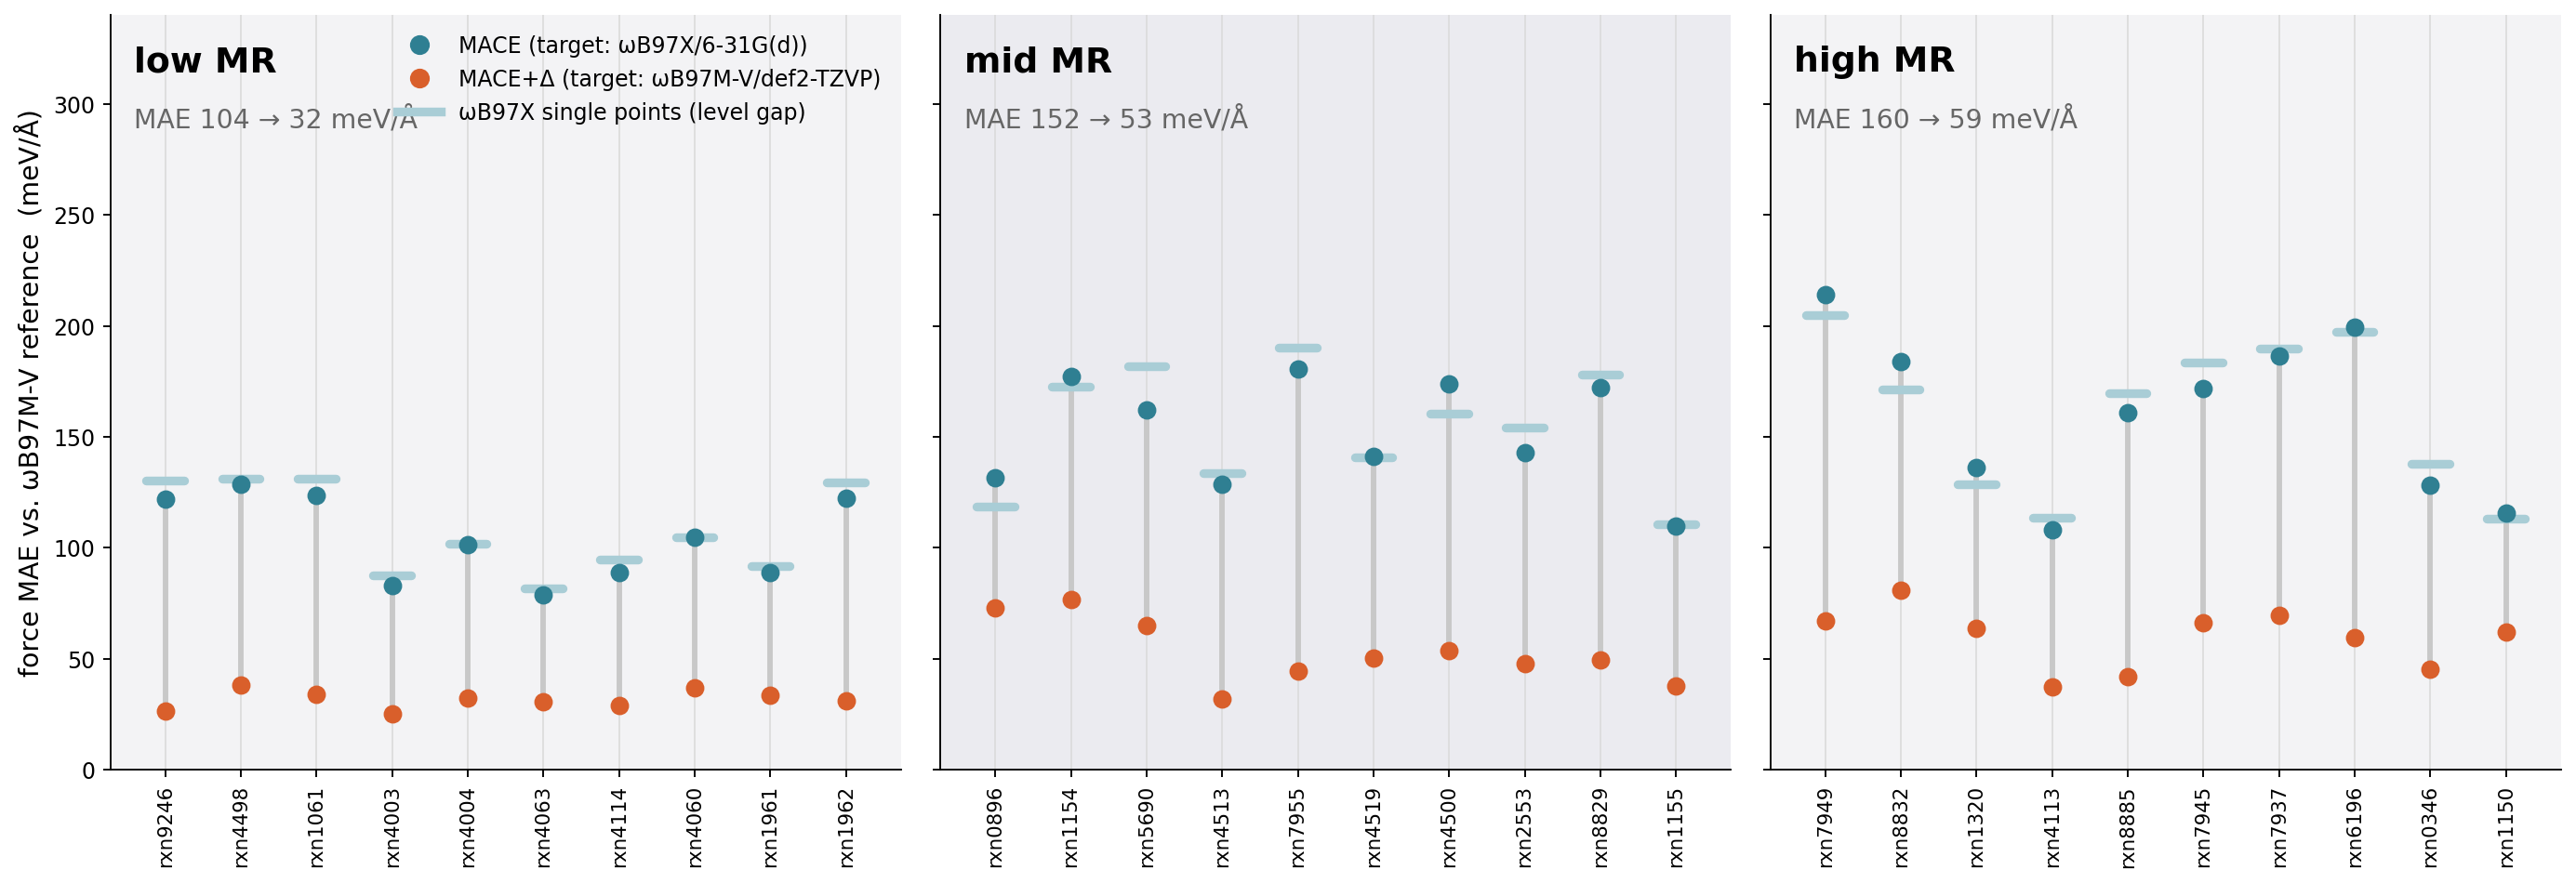
\includegraphics[width=\textwidth]{Pictures/force_errors_dumbbell_v2.png}
  \caption{Force MAE at fixed geometries against the
  $\omega$B97M-V/def2-TZVP reference, per reaction and MR tier. Teal:
  MACE; orange: MACE+$\Delta$; light tick: the $\omega$B97X/6-31G(d)
  single points, which is the level gap itself. MACE sits on the level
  gap almost everywhere, and the correction removes most of it: the
  force error drops on all 30 reactions, in every tier.}
  \label{fig:force-errors}
\end{figure}


\paragraph{Evaluating performance on NEB driven TS search and barrier prediction: how well do the models perform when used end to end?}
In the fixed-geometry evaluation no geometries were optimised; every method was evaluated on
the same fixed reference structures. Now the models do the work themselves:
they relax the endpoints, drive the CI-NEB, and deliver a transition state
and a barrier. All 30 runs converge, with MACE and with MACE+$\Delta$.

We look at the geometries first. All numbers below are Kabsch RMSD
between two transition-state geometries, medians over the 30
reactions. Before asking whether the correction improves the
geometries, we ask how much they could improve at all. Three
distances answer this:

\begin{itemize}
  \item cheap-level DFT transition state to expensive-level DFT
    transition state: 0.007\,\AA{}. This is how far the level upgrade
    moves the transition state, and the most a correction could gain.
  \item MACE transition state to cheap-level DFT transition state:
    0.015\,\AA{}. This is MACE's error against its own level.
  \item MACE transition state to expensive-level reference:
    0.017\,\AA{}. This is MACE's error against the target.
\end{itemize}

MACE's own error is already twice the most the correction could
gain, so it cannot improve the geometries by much; it can only make
them worse. It does not: in Figure~\ref{fig:rmsd-parity} almost all
points lie on the parity line, and the RMSD to the reference goes
from 0.017 to 0.016\,\AA{} in the median and from 0.056 to
0.054\,\AA{} in the mean (Table~\ref{tab:delta-neb-results}).

The barriers repeat the pattern of the fixed-geometry evaluation
(Table~\ref{tab:delta-neb-results}, Figure~\ref{fig:neb-results}). On the
low-MR reactions the error drops from 166 to 52\,meV with near-zero bias.
On the mid- and high-MR reactions the corrected barriers underestimate the
reference by ${\sim}200$\,meV, and on the high tier bare MACE is closer.
The decomposition behind Figure~\ref{fig:bias-decomposition} applies
unchanged: the barriers at the transition states the models found
themselves show the same errors as at the fixed geometries, and no
new one. That the correction improves the low-MR barriers without damaging
the surface is not self-evident, as the next paragraph shows.

\begin{table}[htbp]
  \centering
  \caption{NEB-driven results by MR tier. Barrier error against
  the reference barrier; Kabsch RMSD of the found transition state against
  the reference transition state (mean / median).}
  \label{tab:delta-neb-results}
  \begin{tabular}{llrrc}
    \toprule
    Tier & Method & barrier MAE (meV) & barrier bias (meV) & TS RMSD (\AA) \\
    \midrule
    low  & MACE          & 166.0 & $+166$ & 0.015 / 0.012 \\
         & MACE+$\Delta$ &  52.1 & $+22$  & 0.016 / 0.010 \\
    \midrule
    mid  & MACE          & 233.8 & $+45$  & 0.092 / 0.035 \\
         & MACE+$\Delta$ & 211.6 & $-204$ & 0.065 / 0.034 \\
    \midrule
    high & MACE          &  94.4 & $-3$   & 0.061 / 0.054 \\
         & MACE+$\Delta$ & 236.4 & $-235$ & 0.081 / 0.049 \\
    \midrule
    all 30 & MACE          & 164.7 & $+69$  & 0.056 / 0.017 \\
           & MACE+$\Delta$ & 166.7 & $-139$ & 0.054 / 0.016 \\
    \bottomrule
  \end{tabular}
\end{table}

\begin{figure}[htbp]
  \centering
  
\includegraphics[width=\textwidth]{Pictures/neb_results.png}
  \caption{Barrier errors in the model-driven searches, per reaction
  and MR tier. Top: barrier error of MACE (teal) and MACE+$\Delta$
  (orange) against the $\omega$B97M-V/def2-TZVP reference; triangles
  mark off-scale values. Bottom: the absolute barriers of the same
  reactions, left to right MACE, $\omega$B97M-V/def2-TZVP reference,
  MACE+$\Delta$, each from its own NEB.}
  \label{fig:neb-results}
\end{figure}

\begin{figure}[htbp]
  \centering
  
\includegraphics[width=0.7\textwidth]{Pictures/rmsd_parity.png}
  \caption{Transition-state geometries from the model-driven searches:
  RMSD of the MACE+$\Delta$ transition state against the RMSD of the
  MACE transition state, both measured against the
  $\omega$B97M-V/def2-TZVP transition state, on log axes. The dashed
  line is parity. Points on it mean the correction leaves the geometry
  unchanged, which holds for almost all reactions; the labelled outliers
  are the exceptions, in both directions.}
  \label{fig:rmsd-parity}
\end{figure}

\paragraph{The earlier head.}
Section~\ref{sec:delta-architecture} described the earlier head, whose
active weights sat on rotation-dependent features. To measure the
consequence directly, we rotate each benchmark transition state into 24
random orientations and evaluate $\Delta$ for each. With the earlier head,
$\Delta$ varies by 212\,meV on average and up to 422\,meV; with the
corrected head it varies by less than 0.01\,meV, the level of float32
noise, same as MACE itself. Table~\ref{tab:delta-audit} lists the effect on
the benchmark: the corrected head predicts better forces on all 30
reactions, and it repairs the transition-state geometries. With the earlier
head, NEB found structures twice as far from the reference as bare MACE;
the corrected head restores MACE's geometry quality.

\begin{table}[htbp]
  \centering
  \caption{Earlier head vs.\ corrected head on the 30 benchmark reactions.
  Rotation spread: max$-$min of $\Delta$ over 24 random orientations of the
  transition state, averaged over reactions.}
  \label{tab:delta-audit}
  \begin{tabular}{lrr}
    \toprule
    & earlier head & corrected head \\
    \midrule
    Rotation spread of $\Delta$ (meV) & 212 & $<0.01$ \\
    eMAE, fixed geometries (meV) & 63.7 & 55.6 \\
    fMAE, fixed geometries (meV/\AA) & 76.4 & 48.0 \\
    TS RMSD, NEB-driven (\AA, mean) & 0.101 & 0.054 \\
    Barrier MAE, NEB-driven, low MR (meV) & 89.3 & 52.1 \\
    \bottomrule
  \end{tabular}
\end{table}

% ---- ab hier steht im Entwurf "Protocol B: the surface" + "The earlier head"
% ---- ein zweites Mal, wortgleich inkl. Tabellen und Figuren. In dieser
% ---- Kopie weggelassen; der Text oben ist der vollstaendige Block.

\subsection{Discussion}
\label{sec:delta-discussion}

\paragraph{Overall performance.} Relabelling under 1\,\% of the dataset lifts
the model. The forces improve on every reaction. The energies improve
in every tier. The barriers of the low-MR reactions improve from 170
to 47\,meV at fixed geometries and from 166 to 52\,meV in the
model-driven searches. The geometries stay as good as MACE's. RQ1 is
answered yes.

\paragraph{Dependence on multireference character.} The correction struggles where the
multireference character is high, and the barriers show it most. The
transition state is the point of highest multireference character on
a path, and the barrier is read there. Over the rest of the path the
corrected model is good in every tier.

\paragraph{Origin of the overshoot.} The head does what it was
trained to do in every tier: its error against the true level gap is
$+25$, $-43$ and $+7$\,meV at low, mid and high MR. The overshoot
comes from the base model. MACE misses its own level by $-91$\,meV
at mid MR and by $-192$\,meV at high MR, and that error enters the
corrected barrier unchanged (Figure~\ref{fig:bias-decomposition}).
This is also why bare MACE looks right at high MR: the cheap level
lies $+213$\,meV above the reference, and MACE's own error cancels
most of that gap. MACE lands near the reference by accident, at
$+21$\,meV. The model-driven searches show the same, MACE at
$-3$\,meV and MACE+$\Delta$ at $-235$\,meV
(Table~\ref{tab:delta-neb-results}).

\paragraph{Composition of the benchmark.} The benchmark was built to
expose this. A third of it is the ten reactions with the highest
multireference character in the test split, the top 3.6\,\% of 279.
It did its job. The mid tier is the typical reaction, and there the
barrier error still improves, from 254 to 147\,meV, although its sign
flips. Only at the specifically selected high MR does the correction
make the barriers worse.

\paragraph{Reliability of the reference.} Where the correction
struggles, the reference itself is unreliable. At high
multireference character a restricted determinant describes the
molecule poorly. This chapter cannot check that, because every
calculation in it is restricted. Chapter~\ref{ch:mr} runs the check.
At nine of the ten mid-MR transition states the restricted solution
is the lowest, so the reference is sound and the overshoot there is
an error of the models, mostly the base model's. At seven of the ten
high-MR ones a lower
broken-symmetry solution exists, so the reference was the wrong
target.


% \paragraph{Protocol B: the surface.}
% All 30 NEB runs converge, with MACE and with MACE+$\Delta$.
% Table~\ref{tab:delta-neb-results} shows the outcome. On the low-MR
% reactions the correction does its job: the barrier error drops from 166 to
% 52\,meV, and the transition states the corrected model finds are as close
% to the reference as those of bare MACE (0.016 vs.\ 0.015\,\AA). The
% correction improves the energetics without damaging the surface. On the
% mid- and high-MR reactions the barriers underestimate the reference by
% ${\sim}200$\,meV, as in Protocol A, and on the high tier bare MACE is
% closer to the reference than the corrected model. The geometries suffer far
% less than the barriers: in every tier the found transition states stay
% within 0.1\,\AA{} of the reference.

% \begin{table}[htbp]
%   \centering
%   \caption{Protocol B: NEB-driven results by MR tier. Barrier error against
%   the reference barrier; Kabsch RMSD of the found transition state against
%   the reference transition state (mean / median).}
%   \label{tab:delta-neb-results}
%   \begin{tabular}{llrrc}
%     \toprule
%     Tier & Method & barrier MAE (meV) & barrier bias (meV) & TS RMSD (\AA) \\
%     \midrule
%     low  & MACE          & 166.0 & $+166$ & 0.015 / 0.012 \\
%          & MACE+$\Delta$ &  52.1 & $+22$  & 0.016 / 0.010 \\
%     \midrule
%     mid  & MACE          & 233.8 & $+45$  & 0.092 / 0.035 \\
%          & MACE+$\Delta$ & 211.6 & $-204$ & 0.065 / 0.034 \\
%     \midrule
%     high & MACE          &  94.4 & $-3$   & 0.061 / 0.054 \\
%          & MACE+$\Delta$ & 236.4 & $-235$ & 0.081 / 0.049 \\
%     \bottomrule
%   \end{tabular}
% \end{table}

% \paragraph{The earlier head.}
% Section~\ref{sec:delta-architecture} described the earlier head, whose
% active weights sat on rotation-dependent features. To measure the
% consequence directly, we rotate each benchmark transition state into 24
% random orientations and evaluate $\Delta$ for each. With the earlier head,
% $\Delta$ varies by 212\,meV on average and up to 422\,meV; with the
% corrected head it varies by less than 0.01\,meV, the level of float32
% noise, same as MACE itself. Table~\ref{tab:delta-audit} lists the effect on
% the benchmark: the corrected head predicts better forces on all 30
% reactions, and it repairs the transition-state geometries. With the earlier
% head, NEB found structures twice as far from the reference as bare MACE;
% the corrected head restores MACE's geometry quality. The rough surface was
% a property of the defect, not of the method.

% \begin{table}[htbp]
%   \centering
%   \caption{Earlier head vs.\ corrected head on the 30 benchmark reactions.
%   Rotation spread: max$-$min of $\Delta$ over 24 random orientations of the
%   transition state, averaged over reactions.}
%   \label{tab:delta-audit}
%   \begin{tabular}{lrr}
%     \toprule
%     & earlier head & corrected head \\
%     \midrule
%     Rotation spread of $\Delta$ (meV) & 212 & $<0.01$ \\
%     eMAE, Protocol A (meV) & 63.7 & 55.6 \\
%     fMAE, Protocol A (meV/\AA) & 76.4 & 48.0 \\
%     TS RMSD, Protocol B (\AA, mean) & 0.101 & 0.054 \\
%     Barrier MAE, Protocol B, low MR (meV) & 89.3 & 52.1 \\
%     \bottomrule
%   \end{tabular}
% \end{table}

% \paragraph{The MR limit.}
% Both protocols draw the same line. Where the labels of both levels are
% reliable, the correction works: the barrier error drops by a factor of
% three, at fixed geometries and when the model searches for the transition
% state itself. Where multireference character makes the labels unreliable,
% the correction makes barriers worse than the uncorrected baseline. This is
% a property of delta-learning, not of this head: the head learns the
% difference between two single-reference DFT levels, and where both levels
% are wrong, that difference carries no information about the true surface.
% A correction can only be as good as the labels it learns from. What happens
% on these multireference reactions, and how the corrected model compares to
% models trained natively at the target level, is the subject of
% Chapter~[Y].


% \section{Evaluation protocol}
% \label{sec:delta-protocol}

% Sections~\ref{sec:delta-fixed} and \ref{sec:delta-barriers} hold the geometries fixed.
% Every method is evaluated on the last ten images of the converged ORCA
% \mbox{wB97M-V/def2-TZVP} CI-NEB band for each of the 30 benchmark reactions, giving 300
% structures. No optimisation takes place, so geometry error cannot enter, and the
% comparison isolates the accuracy of the energy and the forces.

% Four conventions are fixed here and used unchanged throughout the chapter.

% \paragraph{Energy anchoring.} Each method's profile is referred to its own first image,
% $\Delta E_m(i) = E_m(i) - E_m(0)$. Constant offsets between levels of theory cancel
% exactly, and the metric measures profile shape only. The error at image 0 is identically
% zero for every method, so nine of the ten images carry information.

% \paragraph{Force error.} The force MAE is a mean over all Cartesian components, not over
% per-atom vector norms. The norm convention would give a systematically larger number
% (roughly $\sqrt{3}$ for isotropic errors) and the two must not be compared.

% \paragraph{Cosine similarity.} Computed per atom, as the angle between the predicted and
% reference three-vector, averaged over all atoms with $|\mathbf{F}| > 10^{-6}$\,eV/\AA{}
% in both structures.

% \paragraph{Aggregation.} Metrics are computed per reaction and then averaged over the 30
% reactions, so each reaction carries equal weight. For energies this coincides with
% pooling, since every reaction contributes ten images; for forces it does not, because
% reactions differ in atom count. The pooled force MAE differs from the reported value by
% 0.4\,meV/\AA.

% \section{Energies and forces at fixed geometry}
% \label{sec:delta-fixed}

% \begin{table}[h]
% \centering
% \caption{Fixed-geometry accuracy against \mbox{wB97M-V/def2-TZVP}, 30 reactions,
% 300 structures. The wB97X column is a level of theory rather than a model, and gives
% the size of the functional and basis gap being corrected. $R^2$ is computed within each
% reaction against the identity and then averaged.}
% \label{tab:delta-fixed}
% \begin{tabular}{lccc}
% \hline
%  & MACE & MACE+delta & wB97X \\
% \hline
% Energy MAE (meV)      & 107.6  & \textbf{63.7}   & 94.9 \\
% Energy bias (meV)     & $+77.4$ & \textbf{$-3.9$} & $+84.8$ \\
% $R^2$                 & 0.9734 & \textbf{0.9899} & 0.9781 \\
% Force MAE (meV/\AA)   & 138.9  & \textbf{76.4}   & 130.9 \\
% Force cosine          & 0.3223 & \textbf{0.5134} & 0.3216 \\
% \hline
% \end{tabular}
% \end{table}

% The energy MAE falls by 41\,\% and the force MAE by 45\,\%. The bias of $+77.4$\,meV is
% removed to within 4\,meV, and $R^2$ increases, so the improvement is not a trade of bias
% against scatter.

% Two of the entries in Table~\ref{tab:delta-fixed} are a check on the premise rather than
% a result. The cosine similarity of bare MACE against \mbox{wB97M-V} (0.3223) equals that
% of \mbox{wB97X} against \mbox{wB97M-V} (0.3216) to three decimals, and the force MAEs
% of the two agree to within 8\,meV/\AA. MACE reproduces the force directions of its
% training level, and its disagreement with \mbox{wB97M-V} is the disagreement between the
% two functionals. What the head adds is the difference between those two columns.

% \section{Barriers at fixed geometry}
% \label{sec:delta-barriers}

% The forward barrier is taken as the maximum of the anchored profile over the ten-image
% band, $E_a = \max_i [E(i) - E(0)]$. This is a discrete band maximum, not an interpolated
% or reoptimised saddle point, so every method is biased low by the same discretisation;
% the bias largely cancels in the comparison because all methods share the geometries.

% \begin{table}[h]
% \centering
% \caption{Forward barrier error at fixed geometry, 30 reactions, in meV. The two
% references answer different questions: \mbox{wB97M-V} is the level the head was trained
% to reproduce, CCSD(T) is an external check.}
% \label{tab:delta-barriers}
% \begin{tabular}{lcccc}
% \hline
%  & \multicolumn{2}{c}{vs \mbox{wB97M-V}} & \multicolumn{2}{c}{vs CCSD(T)} \\
%  & bias & MAE & bias & MAE \\
% \hline
% MACE           & $+114.1$ & 168.4 & $+197.7$ & 226.0 \\
% MACE+delta     & $-33.6$  & \textbf{124.3} & $+50.0$ & \textbf{141.7} \\
% \mbox{wB97M-V} & ---      & ---   & $+83.6$  & 103.8 \\
% \mbox{wB97X} & $+148.2$ & 151.3 & $+231.8$ & 231.8 \\
% \hline
% \end{tabular}
% \end{table}

% The ratio of bias to MAE reads directly as the systematic fraction of the error.
% Against CCSD(T), \mbox{wB97X} sits at $231.8/231.8 = 1.00$: every one of the 30
% reactions errs in the same direction, which is what a pure functional error looks like.
% MACE inherits most of it (0.87). After correction the ratio is 0.35. The head removes
% the systematic component and leaves the reaction-to-reaction variance.

% The head is trained to reproduce \mbox{wB97M-V}, so \mbox{wB97M-V}'s own error against
% CCSD(T) of 103.8\,meV is the lowest value it can reach. Of the 122.2\,meV between MACE
% and that floor, the head recovers 84.3\,meV, or 69\,\%.

% CCSD(T) is a single-reference method (Section~\ref{sec:background-ccsdt}). On reactions
% selected for multireference character it is least reliable exactly where it is most
% needed, and the corresponding entries in Section~\ref{sec:delta-tiers} carry that
% qualification.

% \section{NEB-driven evaluation}
% \label{sec:delta-neb}

% Sections~\ref{sec:delta-fixed} and \ref{sec:delta-barriers} removed geometry error by
% construction. This section restores it. Each model relaxes the endpoints with BFGS to
% $f_{\max} = 0.05$\,eV/\AA, optimises a ten-image band initialised from the Transition1x
% path with plain NEB to $f_{\max} = 0.15$\,eV/\AA, and then runs CI-NEB to
% $f_{\max} = 0.05$\,eV/\AA{} within a 500-step budget. The transition state is the
% highest-energy image of the model's own final band, and geometry agreement is measured
% as the Kabsch RMSD against the ORCA \mbox{wB97M-V} transition state, with proper
% rotations only and fixed atom order.

% \begin{table}[h]
% \centering
% \caption{NEB-driven results, 30 reactions, with the fixed-geometry values of
% Table~\ref{tab:delta-barriers} repeated for comparison. Barrier errors in meV, RMSD
% in \AA.}
% \label{tab:delta-neb}
% \begin{tabular}{lcc|cc}
% \hline
%  & \multicolumn{2}{c|}{NEB-driven} & \multicolumn{2}{c}{fixed geometry} \\
%  & MACE & MACE+delta & MACE & MACE+delta \\
% \hline
% Barrier bias vs \mbox{wB97M-V} & $+69.1$ & $-117.1$ & $+114.1$ & $-33.6$ \\
% Barrier MAE vs \mbox{wB97M-V}  & 164.7   & 173.6    & 168.4    & 124.3 \\
% Barrier MAE vs CCSD(T)         & 212.2   & 167.6    & 226.0    & 141.7 \\
% TS RMSD                        & \textbf{0.056} & 0.101 & --- & --- \\
% \hline
% \end{tabular}
% \end{table}

% The geometry result is unambiguous. Bare MACE places the transition state at 0.056\,\AA{}
% from the ORCA reference and the corrected model at 0.101\,\AA, and the ordering holds in
% every multireference tier (Section~\ref{sec:delta-tiers}), so it is not carried by one
% group of reactions.

% The barrier result depends on the reference. Against \mbox{wB97M-V}, bare MACE is
% marginally better than the corrected model (164.7 against 173.6\,meV); against CCSD(T),
% the corrected model is clearly better (167.6 against 212.2\,meV). The signs explain the
% reversal. Bare MACE overestimates the \mbox{wB97M-V} barrier by 69.1\,meV and the
% corrected model underestimates it by 117.1\,meV, while \mbox{wB97M-V} itself lies
% 83.6\,meV above CCSD(T) (Table~\ref{tab:delta-barriers}). The corrected model's
% underestimate therefore cancels against the reference's overestimate,
% $-117.1 + 83.6 = -33.5$\,meV, which is its bias against CCSD(T). Neither ranking is
% meaningful without naming the reference it is measured against.

% What survives both references is the comparison between the two columns of the same
% model. Driving its own optimisation costs the corrected model 49\,meV against
% \mbox{wB97M-V} and 26\,meV against CCSD(T), while bare MACE loses 3.7\,meV and gains
% 13.8\,meV. The correction transfers to the fixed-geometry barrier and does not transfer
% to the NEB-driven one.

% The NEB-driven bias of the corrected model is $-117.1$\,meV against a fixed-geometry
% value of $-33.6$\,meV: the barriers come out systematically too low, which is consistent
% with the band settling somewhere other than the saddle point. The mechanism is not
% established here.

% The result stands regardless of the mechanism: the same head improves pointwise energies
% and forces and degrades the geometry it converges on. Energy accuracy and geometry
% accuracy are two properties of a model, and this head has them moving in opposite
% directions.

% \paragraph{Convergence.} All 30 runs of both models wrote a convergence marker, and both
% reached $f_{\max} \leq 0.05$\,eV/\AA{} on 24 of 30. Six runs terminated with $f_{\max}$
% between 0.064 and 0.132\,eV/\AA{} after 447--772 optimiser steps, while every other run
% finished within 434 steps; the step counter carries across both NEB phases, so the CI-NEB
% phase receives what remains of the 500-step budget rather than a fresh one, and these six
% exhausted it. Five of the six are the same reactions for both models. The defensible
% statement is that 30/30 terminated with a marker and 24/30 additionally reached
% $f_{\max} \leq 0.05$\,eV/\AA. Two of the six, \texttt{rxn7949} and \texttt{rxn7937}, are
% high-MR reactions, so the high-tier NEB numbers below rest in part on bands that did not
% converge.

% The correction changes the cost of the optimisation, not its convergence behaviour. The
% corrected model takes more steps than bare MACE on 25 of 30 reactions, with a median
% ratio of 2.2 and a total of 5352 against 4142 steps, a factor of 1.29 overall. The mean
% of the per-reaction ratios is 15.9, which is dominated by reactions where bare MACE
% converged in one to four steps and is not a useful summary.

% \section{Stratification by multireference character}
% \label{sec:delta-tiers}

% The 30 benchmark reactions were ranked by $N_{\text{FOD}}$
% (Section~\ref{sec:background-mr-diagnostics}) and split into three tiers of ten:
% ranks 1--10 high, 11--20 mid, 21--30 low. No metric definition changes between tiers;
% only the subset does.

% \begin{table}[h]
% \centering
% \caption{Fixed-geometry metrics by FOD tier, MACE $\rightarrow$ MACE+delta, $n = 10$
% per tier. Energy and force MAE in meV and meV/\AA{} against \mbox{wB97M-V}; barrier MAE
% in meV against the \mbox{wB97M-V} NEB barrier.}
% \label{tab:delta-tiers}
% \begin{tabular}{lccc}
% \hline
% tier & energy MAE & force MAE & barrier MAE \\
% \hline
% high & $88.7 \rightarrow 73.5$  & $160.4 \rightarrow 87.0$ & $81.2 \rightarrow 150.9$ \\
% mid  & $148.2 \rightarrow 70.0$ & $151.9 \rightarrow 80.1$ & $254.0 \rightarrow 135.8$ \\
% low  & $86.0 \rightarrow 47.6$  & $104.2 \rightarrow 62.0$ & $169.9 \rightarrow 86.4$ \\
% \hline
% \end{tabular}
% \end{table}

% Energies and forces improve in all three tiers. Barriers improve in the mid and low
% tiers and degrade in the high tier, where bare MACE has the lowest error of the three
% methods.

% The same split appears in the NEB-driven barriers against \mbox{wB97M-V}, where bare
% MACE gives 94.4, 233.8 and 166.0\,meV for the high, mid and low tier and the corrected
% model gives 272.1, 159.4 and 89.3\,meV. Bare MACE is better on the high tier by a factor
% of 2.9 and worse on the other two. It is also closer in transition-state RMSD in every
% tier (0.061, 0.092, 0.015\,\AA{} against 0.134, 0.116, 0.053\,\AA).

% Bare MACE's high-tier barrier MAE of 81.2\,meV is its lowest of the three tiers and lies
% below \mbox{wB97X}'s 124.4\,meV on the same reactions. Its energy MAE on that tier
% (88.7\,meV) is not correspondingly low. The two are not consistent with each other and
% the discrepancy is not resolved here.

% Against CCSD(T), the high tier gives MACE 238.8, MACE+delta 175.5 and \mbox{wB97M-V}
% itself 225.8\,meV. The corrected model does not outperform its own training target;
% CCSD(T) is the least reliable yardstick on precisely these reactions, and no argument is
% built on this ordering.

% The tier pattern is consistent with the scope of the correction. The head learns the
% difference between two single-reference functionals. Where the \mbox{wB97X} labels
% are themselves unreliable, that difference is not the quantity that needs correcting.
% The head does not become useless there, as the energy and force columns show, but the
% improvement stops converting into better barriers.

% With $n = 10$ per tier and no confidence intervals, barrier MAEs are sensitive to single
% reactions, and tier-to-tier differences below the spread of individual reaction errors
% are not resolved.

% \section{Comparison with models trained at the reference level}
% \label{sec:delta-omol}

% The delta head reaches \mbox{wB97M-V} accuracy by correcting a model trained elsewhere.
% The alternative is to train on \mbox{wB97M-V}-level data directly, which is what the
% OMol25 dataset~\cite{omol25} provides and what UMA~\cite{uma} and eSEN~\cite{esen} are
% trained on. This section places the head against that alternative.

% The comparison uses the 22 benchmark reactions for which the restricted Kohn--Sham
% solution is the stable SCF solution. On the remaining reactions the
% \mbox{wB97M-V/def2-TZVP} reference is not the electronic ground state
% (Section~\ref{sec:background-stability}), and a deviation from it measures a property of
% the reference rather than of the model. Restricting to the stable subset removes that
% term. The tier labels used elsewhere in this chapter do not carry over to this subset and
% are not used here. Geometries, metrics and conventions are otherwise those of
% Section~\ref{sec:delta-protocol}.

% \begin{table}[h]
% \centering
% \caption{Fixed-geometry accuracy on the 22 RKS-stable reactions, evaluated against both
% levels of theory. Energy MAE in meV, force MAE in meV/\AA.}
% \label{tab:delta-omol}
% \begin{tabular}{lcc|cc}
% \hline
%  & \multicolumn{2}{c|}{vs \mbox{wB97M-V}} & \multicolumn{2}{c}{vs \mbox{wB97X}} \\
%  & energy & force & energy & force \\
% \hline
% UMA-S       & \textbf{5.1} & 11.5 & 99.4 & 131.1 \\
% UMA-M       & 5.3 & \textbf{10.8} & 99.9 & 130.8 \\
% eSEN        & \textbf{4.9} & 12.7 & 99.3 & 131.2 \\
% MACE+delta  & 62.1 & 72.4 & 111.1 & 143.5 \\
% MACE        & 109.3 & 130.6 & \textbf{41.5} & \textbf{33.4} \\
% \mbox{wB97X} & 98.8 & 130.9 & --- & --- \\
% \hline
% \end{tabular}
% \end{table}

% Read across the rows rather than down the columns. UMA-S disagrees with
% \mbox{wB97X} by 99.4\,meV and 131.1\,meV/\AA; the two functionals disagree with each
% other by 98.8\,meV and 130.9\,meV/\AA. The same holds for UMA-M and eSEN. Their
% disagreement with \mbox{wB97X} is the functional gap, which places them on the
% \mbox{wB97M-V} surface. MACE shows the mirror image against its own training level
% (41.5\,meV, cosine 0.955). Each model reproduces the level of theory it was trained on.

% Relative to bare MACE's 109.3\,meV, the delta head closes 43\,\% of the distance to the
% reference and the OMol25-trained models close 95\,\%. The models also have no failure
% cases on this set: their worst single-reaction energy MAEs are 12.2, 12.4 and 8.9\,meV,
% against 181.6\,meV for MACE+delta and 281.9\,meV for MACE.

% This is not an architecture comparison. UMA and eSEN are evaluated at the level of theory
% they were trained on and MACE is not, so the quantity being measured is what the training
% data provides. Two further points bear on how far the numbers can be pushed. OMol25 uses
% def2-TZVPD, while the reference here is def2-TZVP, so the models reach these values
% across a basis mismatch. Charge and spin were left at the fairchem defaults, neutral
% closed-shell singlet, which is correct for this set and is a default rather than an
% assertion. The relationship between the OMol25 training data and Transition1x is taken up
% in Chapter~\ref{ch:reference}.

% Cosine similarity is not informative in this regime. The OMol25 models score 0.82--0.84
% despite force MAEs an order of magnitude better than MACE's 0.955 against its own level,
% because once the errors are small the residual concentrates on atoms with near-zero
% forces, whose direction is ill-defined.

% \section{Limitations}
% \label{sec:delta-limitations}

% \paragraph{The correction is a functional and basis correction.} It targets the gap
% defined in Equation~\ref{eq:delta-def} and nothing else. Where the \mbox{wB97X}
% labels are unreliable for reasons of multireference character, the head has no access to
% that error, and Section~\ref{sec:delta-tiers} shows where this becomes visible.

% \paragraph{The offset is removed, the variance is not.} The bias against CCSD(T) falls
% from 0.87 of the MAE to 0.35. What remains is reaction-to-reaction scatter that is not
% predictable from the features the head sees.

% \paragraph{Pointwise accuracy does not imply a better optimisation surface.} The head
% improves energies and forces at fixed geometry and degrades the transition-state
% geometries obtained by driving NEB with it. In its present form it should be used to
% evaluate energies on geometries produced by another method, not to produce the
% geometries.

% \paragraph{Generalisation across reactions is the limiting factor.} $\Delta$ is smooth
% within a reaction and varies between reactions. The head is asked to transfer a
% geometry-dependent correction to reactions it has not seen, and the residual error is
% concentrated there.

% \paragraph{Training and evaluation geometries differ in origin.} The head is trained on
% Transition1x \mbox{wB97X} path geometries and evaluated on ORCA \mbox{wB97M-V} path
% geometries. Both are reaction-path structures and the evaluation is closer to deployment
% for it, but it is not an in-distribution test.

% \section{Summary}
% \label{sec:delta-summary}

% A 65\,600-parameter readout head on a frozen MACE backbone, trained on 80\,592 labelled
% geometries, moves fixed-geometry energies from 107.6 to 63.7\,meV and forces from 138.9
% to 76.4\,meV/\AA{} against \mbox{wB97M-V/def2-TZVP}, and recovers 69\,\% of the
% achievable improvement in barrier heights against CCSD(T). Driving NEB with the same
% head raises the barrier error from 124.3 to 173.6\,meV against \mbox{wB97M-V} and the
% transition-state RMSD from 0.056 to 0.101\,\AA{} relative to bare MACE. Against CCSD(T)
% the corrected model retains an advantage over bare MACE in the NEB-driven barriers
% (167.6 against 212.2\,meV), so the barrier ranking depends on the reference; the geometry
% ranking does not. The improvement is confined to the energy, and the degradation is
% confined to the geometry.

% The tier analysis marks the boundary of the correction: it works where the training
% labels are reliable and stops converting into better barriers where they are not. That
% boundary is where Chapter~\ref{ch:reference} begins.